\chapter{Mechanischer Aufbau}
\label{cha:Mechanischer Aufbau}

%Je nach Art der Arbeit kann diese Kapitelüberschrift auch \glqq Ergebnisse\grqq~lauten, z.~B. bei rein messtechnischen Aufgaben.

%Beschreibung der Umsetzung des zuvor gewählten Vorgehens (theoretische Untersuchung, Erhebungen, Durchführung von Experimenten, Prototypenaufbau, Implementierung eines Prozesses, etc.).

%Verifikation anhand der zuvor erarbeiteten Anforderungen und Validierung in Bezug auf das zuvor gestellte Ziel. Diskussion der Ergebnisse. Spätestens hier auch auf die Zuverlässigkeit der gewonnenen Erkenntnisse eingehen (z.~B. anhand der Genauigkeit von Messergebnissen).

Für die Umsetzung des 4-Gewinnt-Roboters wurde eine mechanische Konstruktion gewählt, die es erlaubt, das Spielfeld zu scannen sowie Chips gezielt in eine Spalte einzuwerfen. Der Aufbau umfasst drei Winkelmotoren, einen Farbsensor und einen Drucktaster. Im Folgenden werden die einzelnen Komponenten detailliert beschrieben. Dabei beziehen sich die Ziffern der Aufzählung der einzelnen Sensoren und Aktoren auf die Abbildung 4.1 und Abbildung 4.2.

Die mechanische Konstruktion basiert auf die Idee einem kartesischen Koordinatensystem, bei dem der Farbsensor durch die Kombination aus horizontaler und vertikaler Bewegung jede Spielfeldposition präzise anfahren kann. Das System erlaubt eine vollautomatische Spielweise.

\section{Einbindung von Aktorik}
\begin{enumerate}
	\item \textbf{Horizontalantrieb}\\
	Der horizontale Antrieb des Farbsensors erfolgt über einen Winkelmotor. Dieser ist dafür zuständig, die Spielfeldspalten nacheinander anzufahren. Der Motor ist mit einer Achse verbunden, welche zwei Räder antreiben. Die Bewegung erfolgt in gleichmäßigen Schritten: Eine Drehung um exakt 72 Grad bewegt den Roboter um eine Spalte weiter. Diese Schrittweite wurde so gewählt, dass sie der Breite einer Spalte im Spielfeld entspricht. Dadurch ist eine exakte Positionierung des Sensors über jeder Spalte möglich, ohne dass zusätzliche Sensoren zur Positionsbestimmung notwendig sind. 
	\item \textbf{Vertikalantrieb}\\
	 Um das Spielfeld auch in vertikaler Richtung abfahren zu können, ist der Farbsensor an einer Kette montiert. Diese Kette wird durch einen Winkelmotor angetrieben. Der Sensor ist an einem mittleren Segment der Kette befestigt und fährt beim Drehen der Kette entsprechend auf und ab. Ein Schritt des Motors um 95 Grad bewegt den Sensor um genau eine Spielfeldhöhe weiter. Auf diese Weise können sämtliche sechs Reihen der aktuellen Spalte nacheinander abgescannt werden. Die Rückwärtsbewegung der Kette erlaubt es, den Sensor wieder nach unten zu fahren.
	\item \textbf{Chipauswerfer}\\
	Das Einwerfen des eigenen Spielsteins erfolgt ebenfalls über einen Winkelmotor. An diesem Motor ist eine Stange montiert, die bei einer vollständigen Umdrehung einen Spielchip aus dem Vorratsmagazin (mit der Software Fusion360 konstrukiert und 3D-gedruckt) in die gewünschte Spalte stößt. Nach der Auslösung kann ein neuer Chip in die Abschussposition nachrutschen. In der Software ist eine Wartezeit nach dem Auslösen eingebaut, damit der Chip sicher im Spielfeld ankommt, bevor die nächste Aktion beginnt.


\section{Einbindung von Sensorik}

	\item \textbf{Startsignal}\\
	Um dem Roboter mitzuteilen, dass er den nächsten Zug starten kann wurde ein Kraftsensor angebracht. Dieser befindet sich an der Vorderseite des Roboters. Sobald der Spieler den Sensor leicht berührt, wird ein Signal ausgelöst und der Prozess startet. 
	\item \textbf{Spielfeldscan – Farbsensor an Kette}\\
	 Für die Farberkennung des Spielfeldes wurde ein LEGO-Farbsensor verwendet, der über die oben beschriebene Kettenkonstruktion vertikal verfahrbar ist. Die Farbmessung erfolgt jeweils in der Mitte eines Spielfeldes. Der Sensor erkennt RGB-Werte (in diesem Projekt benutzt: Rot, Gelb oder Leer). Der Abstand zwischen Sensor und Spielfeld beträgt etwa 7 mm. Dieser Wert hat sich als optimal für zuverlässige Farbmessung erwiesen.
\end{enumerate}


\begin{figure}[H]
	\centering
	\begin{minipage}[b]{0.48\linewidth}
		\centering
		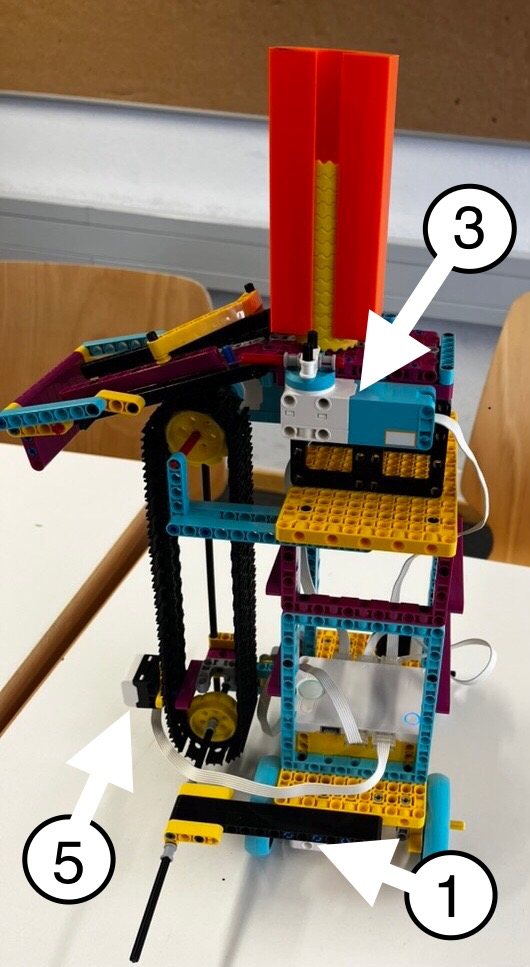
\includegraphics[width=\linewidth]{images/188CF006-D571-4F2D-9337-8C4BDD7DAAEF_1_105_c}
		\caption{Seitenansicht links}
		\label{fig:seitenansicht-links}
	\end{minipage}
	\hfill
	\begin{minipage}[b]{0.48\linewidth}
		\centering
		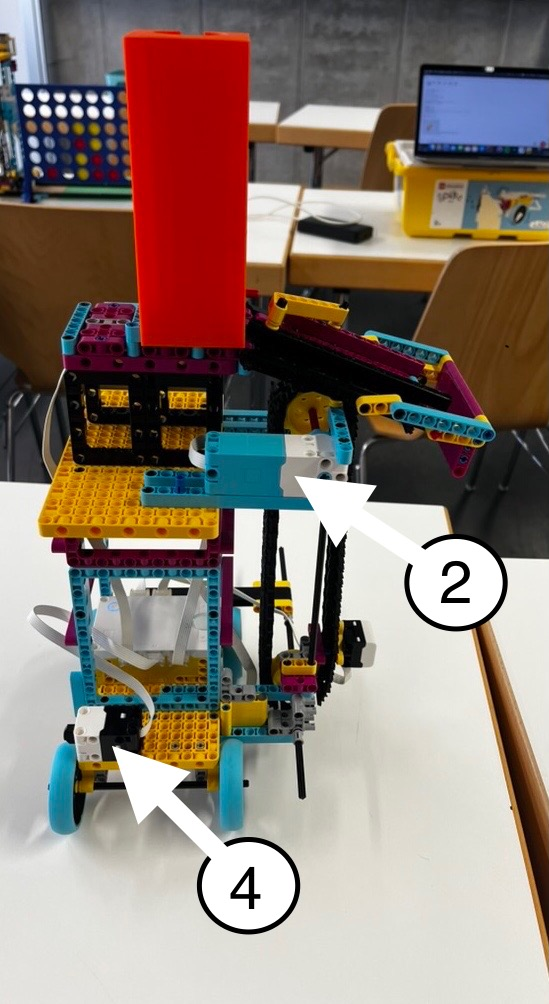
\includegraphics[width=\linewidth]{images/DAE26A50-277E-4C6B-96A3-F2DE2CC9C004_1_105_c}
		\caption{Seitenansicht rechts}
		\label{fig:seitenansicht-rechts}
	\end{minipage}
\end{figure}


\section{Software}
Im Kapitel Software wird genauer beschrieben, wie die Programmierung des Vier-Gewinnt-Roboters umgesetzt ist. Die Software bildet das Kernstück des Roboters und ist entscheidend dafür, dass dieser eigenständig am Spiel teilnehmen kann.



\tikzstyle{startstop} = [ellipse, draw, fill=gray!10, minimum width=3cm, minimum height=1cm]
\tikzstyle{io} = [trapezium, trapezium left angle=70, trapezium right angle=110, draw, fill=blue!10, minimum width=3cm, minimum height=1cm]
\tikzstyle{process} = [rectangle, draw, fill=orange!10, minimum width=3cm, minimum height=1cm]
\tikzstyle{decision} = [diamond, draw, fill=green!10, aspect=2, minimum width=3cm, minimum height=1cm]
\tikzstyle{arrow} = [thick,->,>=Stealth]

\begin{figure}[H]

\begin{tikzpicture}[node distance=2cm]
	\node (start) [startstop] {Start};
	\node (wait) [process, below of=start] {Warten auf Sensor-Aktivierung};
	\node (move) [process, below of=wait] {Spielfeld anfahren};
	\node (scan) [process, below of=move] {Spalten scannen};
	\node (update) [process, below of=scan] {Board-Update};
	\node (opponent) [decision, below of=update, yshift=-0.7cm] {Neuer gegnerischer Stein?};
	\node (calc) [process, below of=opponent, yshift=-0.7cm] {Optimalen Zug berechnen (Alpha-Beta)};
	\node (motor) [process, below of=calc] {Motorsteuerung: Stein platzieren};
	\node (win) [decision, below of=motor, yshift=-0.7cm] {Gewonnen?};
	\node (congrats) [startstop, right of=win, xshift=5cm] {Glückwunsch! Spiel gewonnen};
	\node (print) [process, below of=win] {Spielfeld ausgeben};

	
	\draw [arrow] (start) -- (wait);
	\draw [arrow] (wait) -- (move);
	\draw [arrow] (move) -- (scan);
	\draw [arrow] (scan) -- (update);
	\draw [arrow] (update) -- (opponent);
	\draw [arrow] (opponent) -- node[right] {Ja/Nein} (calc);
	\draw [arrow] (calc) -- (motor);
	\draw [arrow] (motor) -- (win);
	\draw [arrow] (win) -- node[above] {Ja} (congrats);
	\draw [arrow] (win) -- node[right] {Nein} (print);
	\draw [arrow] (congrats) |- (print);
	\draw [arrow] (print.west) -| ($(wait.west)+(-1.5,0)$) -- (wait.west);
	
\end{tikzpicture}

	\caption[Flussdiagramm]{Flussdiagramm der Software}
\label{fig:Flussdiagramm}
\end{figure}
\chapter{Programmlogik}

In diesem Kapitel wird die Softwarestruktur des 4-Gewinnt-Roboters systematisch beschrieben. Da der vollständige Quellcode eine Vielzahl an Funktionen, Hilfsroutinen und technischen Details umfasst, wird in diesem Kapitel aus Gründen der Übersichtlichkeit nicht jede einzelne Codezeile dargestellt und erläutert.
Stattdessen liegt der Fokus auf den wesentlichen Programmabschnitten, die das Spielverhalten maßgeblich bestimmen.

Zur besseren Nachvollziehbarkeit der Funktionsweise wird die Darstellung in zwei Teile gegliedert:

\begin{itemize}
	\item Zunächst wird der \textbf{Algorithmus zur Spielentscheidung} detailliert erläutert. Dabei handelt es sich um den Minimax-Algorithmus mit Alpha-Beta-Pruning. Dieser Abschnitt behandelt ausschließlich die Entscheidungslogik.
	
	\item Im Anschluss wird das \textbf{Hauptprogramm} vorgestellt, das alle Bestandteile miteinander verknüpft. Es steuert den Ablauf des Spiels von der Spielerkennung über das Spielfeld-Scanning bis zur Ausführung des eigenen Spielzugs. Dabei werden sowohl Sensoren als auch Motoren angesprochen und der Entscheidungsalgorithmus eingebunden.
\end{itemize}

Diese Zweiteilung erlaubt es, sowohl die algorithmische Tiefe als auch die technische Umsetzung getrennt zu betrachten und anschließend im Gesamtkontext zu verstehen.

Desweiteren wird im Unterkapitel 5.3 die konkrete Umsetzung der Spielsteuerung und Entscheidungslogik für den 4-Gewinnt-Roboter beschrieben. Der Fokus liegt auf der softwareseitigen Realisierung unter Berücksichtigung der limitierten Hardware-Ressourcen des LEGO Spike Prime Hubs. Es werden hierbei zentrale Entwurfsentscheidungen erläutert.


\section{Algorithmus}

Ein zentraler Bestandteil des 4-Gewinnt-Roboters ist die Entscheidungsfindung durch einen algorithmischen Spielbaum. Dieser wird mit dem bekannten\newline Minimax-Algorithmus unter Verwendung von Alpha-Beta-Pruning realisiert. Ziel ist es, basierend auf dem aktuellen Spielfeldzustand den optimalen Zug für die KI zu berechnen.
Der Algorithmus bewertet mögliche Züge bis zu einer bestimmten Tiefe im Spielbaum und trifft Entscheidungen, die langfristig zum Sieg führen können oder gegnerische Gewinnzüge verhindern.

\textbf{Spielfeld und Spielerdefinition}
Im Vorfeld des Algorithmus ist festgelegt, welches Symbol der Algorithmus (die KI) spielt:

\begin{lstlisting}[style=pythonstyle]
	my_piece = 1  # 1 = YELLOW (AI player), -1 = RED
	opponent_piece = -my_piece
\end{lstlisting}

Dabei entspricht 1 dem gelben Spielstein (der KI), -1 dem roten Spielstein (dem Gegner). Diese numerische Darstellung vereinfacht die Bewertung und das Vergleichen der Felder im Spielfeld.

\textbf{Bewertungsfunktion}
Der Algorithmus benötigt eine Bewertungsfunktion, die die Qualität eines Spielzustands abschätzt. Dies geschieht durch eine Heuristik, die mögliche Gewinnlinien zählt und bewertet.
Die Bewertungsfunktion basiert auf der Idee, sogenannte „Fenster“ (Ausschnitte aus 4 Feldern) im Spiel zu analysieren und zu beurteilen, wie viele Steine der KI bzw. des Gegners in diesen Fenstern enthalten sind:

\begin{lstlisting}[style=pythonstyle]
	def evaluate_window(window, player):
	opp_player = opponent_piece if player == my_piece else my_piece
	score = 0
	if window.count(player) == 4:
	score += 100
	elif window.count(player) == 3 and window.count(0) == 1:
	score += 5
	elif window.count(player) == 2 and window.count(0) == 2:
	score += 2
	if window.count(opp_player) == 3 and window.count(0) == 1:
	score -= 4
	return score
\end{lstlisting}

Diese Funktion bewertet sowohl offensive als auch defensive Situationen. Ein Fenster mit drei eigenen Steinen und einem leeren Feld wird positiv bewertet, ein Fenster mit drei gegnerischen Steinen und einem leeren Feld hingegen negativ, um Bedrohungen abzuwehren.

Die Hauptfunktion zur Bewertung des gesamten Spielfeldes aggregiert alle horizontalen, vertikalen und diagonalen Fenster:

\begin{lstlisting}[style=pythonstyle]
	def evaluate(board):
	score = 0
	center_array = [board[r][field_width//2] for r in range(field_height)]
	center_count = center_array.count(my_piece)
	score += center_count * 3
\end{lstlisting}

Zunächst werden die mittleren Spalten stärker gewichtet, da sie strategisch wichtiger sind (siehe Teil 1 xxxxx)

Anschließend werden alle Zeilen, Spalten und Diagonalen analysiert:

\begin{lstlisting}[style=pythonstyle]
	for r in range(field_height):
	row_array = [board[r][c] for c in range(field_width)]
	for c in range(field_width - 3):
	window = row_array[c:c+4]
	score += evaluate_window(window, my_piece)
	score -= evaluate_window(window, opponent_piece)
\end{lstlisting}

Diese Schleifen bilden das heuristische Fundament für die spätere Entscheidungsfindung.

\textbf{Minimax mit Alpha-Beta-Pruning}

Die Hauptentscheidung trifft der Minimax-Algorithmus. Dabei wird rekursiv der Spielbaum aufgebaut, wobei sich der Algorithmus abwechselnd in die Rolle der KI („maximizing player“) und des Gegners („minimizing player“) versetzt. Um die Effizienz zu steigern, wird Alpha-Beta-Pruning genutzt. Dabei werden Äste im Spielbaum verworfen, wenn sie nachweislich zu schlechteren Ergebnissen führen. (siehe Teil 1 xxx)

Der Einstiegspunkt ist:

\begin{lstlisting}[style=pythonstyle]
	def alpha_beta(board, depth, alpha, beta, maximizing_player):
\end{lstlisting}

Zuerst wird geprüft, ob der aktuelle Zustand bereits im Transposition Table gespeichert ist – einem Cache zur Vermeidung redundanter Berechnungen:

\begin{lstlisting}[style=pythonstyle]
	key = (board_hash(board, maximizing_player), depth)
	if key in transposition_table:
	return transposition_table[key]
\end{lstlisting}

Anschließend erfolgt eine Prüfung: Ist der Zug eine Gewinnsituation, oder wurde die maximale Tiefe erreicht?

\begin{lstlisting}[style=pythonstyle]
	valid_locations = [col for col in range(field_width) if is_valid_location(board, col)]
	terminal = winning_move(board, my_piece) or winning_move(board, opponent_piece) or len(valid_locations) == 0
	if depth == 0 or terminal:
	...
\end{lstlisting}

Falls ja, gibt die Funktion eine Bewertung zurück. Andernfalls wird der Spielbaum weiter durchlaufen.

\textbf{Maximierender Spieler (KI)}

\begin{lstlisting}[style=pythonstyle]
	if maximizing_player:
	value = -float('inf')
	for col in valid_locations:
	...
	new_score = alpha_beta(..., False)[1]
	if new_score > value:
	value = new_score
	best_col = col
	alpha = max(alpha, value)
	if alpha >= beta:
	break
\end{lstlisting}

Hier versucht der Algorithmus, die maximal erreichbare Bewertung zu finden und prüft regelmäßig, ob das aktuelle Ergebnis besser ist als die bisherige beste Option. Wenn \texttt{alpha >= beta}, wird der restliche Baum abgeschnitten (Pruning).

\textbf{Minimierender Spieler (Gegner)}

Analog erfolgt das Vorgehen für den Gegner:

\begin{lstlisting}[style=pythonstyle]
	else:
	value = float('inf')
	for col in valid_locations:
	...
	new_score = alpha_beta(..., True)[1]
	if new_score < value:
	value = new_score
	best_col = col
	beta = min(beta, value)
	if beta <= alpha:
	break
\end{lstlisting}

Am Ende wird das Ergebnis in der Transpositionstabelle gespeichert und zurückgegeben:

\begin{lstlisting}[style=pythonstyle]
	transposition_table[key] = result
	return result
\end{lstlisting}

\subsection{Dynamische Suchtiefe}

Je nach Spielphase kann es sinnvoll sein, tiefer oder flacher zu suchen. Zu Beginn reicht eine niedrige Tiefe, da viele Züge möglich sind. In späteren Phasen erhöht sich die Tiefe:

\begin{lstlisting}[style=pythonstyle]
	def get_dynamic_depth(board):
	empty = sum(row.count(0) for row in board)
	if empty > 30:
	return 3
	else:
	return 4
\end{lstlisting}

Diese dynamische Anpassung balanciert Spielstärke und Rechenzeit optimal.

\textbf{Fazit}

Der eingesetzte Minimax-Algorithmus mit Alpha-Beta-Pruning stellt das strategische Herzstück des 4-Gewinnt-Roboters dar. Durch gezielte Bewertung von Spielpositionen, Berücksichtigung gegnerischer Drohungen und dynamische Tiefenanpassung kann der Roboter selbstständig Züge planen, Gefahren abwehren und letztlich siegreich agieren. Die Verwendung eines Transpositionstables beschleunigt dabei die Entscheidungsfindung, indem bereits analysierte Spielsituationen nicht erneut bewertet werden müssen. Das Ergebnis ist ein hochgradig effektives Entscheidungsverfahren für ein strategisches Spiel wie 4-Gewinnt.


\section{Ablaufsteuerung des Hauptprogramms}

Nachdem der Algorithmus erläutert wurden und in Kapitel xxx die Konstruktion und Ansteuerung des Roboters aufgezeigt wurde, beschreibt dieses Kapitel den Gesamtablauf des Programms. Dabei steht im Fokus, wie die Spielfelderkennung, Algorithmus und Ausführungsschritte zu einem vollständigen Spielzug kombiniert werden.

\textbf{Initialisierung}:
Zu Beginn wird das Spielfeld als leere Matrix angelegt. Zusätzlich wird eine Kopie gespeichert, um Änderungen im Vergleich zur vorherigen Runde erkennen zu können.

\begin{lstlisting}[style=pythonstyle]
	board = [[0 for _ in range(field_width)] for _ in range(field_height)]
	last_board = [row[:] for row in board]
\end{lstlisting}

\textbf{Warten auf Eingabe durch den Spieler}

Bevor der Roboter mit dem Scannen des Spielfeldes beginnt, wartet er auf eine Aktivierung des Drucksensors am Port C.

\begin{lstlisting}[style=pythonstyle]
	print("Waiting for sensor at port C...")
	while not sensor_activated():
	time.sleep(0.1)
\end{lstlisting}

\textbf{Positionierung an der Startspalte}

Der Roboter fährt seine Sensorplattform an die rechte Spielfeldseite (Spalte 6), um von dort den Scan zu beginnen.

\begin{lstlisting}[style=pythonstyle]
	motor.run_for_degrees(port.D, 198, 170)
	time.sleep(1.5)
\end{lstlisting}

\textbf{Scannen des Spielfelds}

Von rechts nach links wird jede Spalte analysiert. Dabei wird der Farbsensor in die erste freie Zeile der Spalte bewegt:

\begin{lstlisting}[style=pythonstyle]
	motor.run_for_degrees(port.E, move_distance_e * (free_row), speed_E)
	detected_color = color_sensor.color(port.B)
	update_board(free_row, matrix_col, detected_color)
	motor.run_for_degrees(port.E, -move_distance_e * free_row, speed_E)
\end{lstlisting}

Wird ein neuer gegnerischer Spielstein erkannt, wird seine Position gespeichert und der Scan abgebrochen:

\begin{lstlisting}[style=pythonstyle]
	if (last_board[free_row][matrix_col] == 0 and
	board[free_row][matrix_col] == opponent_piece):
	opponent_piece_found = True
	opponent_col = col
\end{lstlisting}

\textbf{Berechnung des Spielzugs}

Die Tiefe der Suche wird dynamisch abhängig vom Spielstand gewählt. Anschließend wird der beste Spielzug mit Minimax und Alpha-Beta-Pruning berechnet:

\begin{lstlisting}[style=pythonstyle]
	dynamic_depth = get_dynamic_depth(board_numeric)
	
	best_col, _ = alpha_beta(
	board_numeric,
	depth=dynamic_depth,
	alpha=-float('inf'),
	beta=float('inf'),
	maximizing_player=(my_piece == 1)
	)
\end{lstlisting}

\textbf{Ausführen des Spielzugs}

Zuerst wird die physische Zielspalte berechnet und der Roboter dorthin bewegt:

\begin{lstlisting}[style=pythonstyle]
	physical_target_col = field_width - 1 - best_col
	motor.run_for_degrees(port.D, -move_distance_d * physical_target_col, speed_D)
\end{lstlisting}

Danach wird ein Spielstein mithilfe des Motors A ausgeworfen:

\begin{lstlisting}[style=pythonstyle]
	motor.run_for_degrees(port.A, -360, speed_A)
	time.sleep(3)
\end{lstlisting}

Das Spielfeld wird nach dem Wurf aktualisiert:

\begin{lstlisting}[style=pythonstyle]
	board[best_row][best_col] = my_piece
	last_board = [row[:] for row in board]
\end{lstlisting}

Anschließend erfolgt eine Prüfung auf einen möglichen Spielsieg:

\begin{lstlisting}[style=pythonstyle]
	if winning_move(board, my_piece):
	print(" Congratulations! The robot has WON the game!")
	print_board(board)
	sound.beep(440, 1000000, 100)
	break
\end{lstlisting}

\textbf{Zurückfahren in Ausgangsposition}

Unabhängig vom Spielausgang kehrt der Roboter an seine Startposition zurück:

\begin{lstlisting}[style=pythonstyle]
	motor.run_for_degrees(port.D, -199, speed_D)
\end{lstlisting}

\textbf{Warten auf die nächste Runde}

Abschließend wird auf das Loslassen des Drucksensors gewartet, bevor ein neuer Zyklus beginnt:

\begin{lstlisting}[style=pythonstyle]
	while sensor_activated():
	time.sleep(0.1)
\end{lstlisting}

\textbf{Fazit}

Die Ablaufsteuerung des Hauptprogramms ist zyklisch aufgebaut und gewährleistet einen strukturierten Spielverlauf: Der Roboter wartet auf das Startsignal, scannt das Spielfeld, berechnet den optimalen Spielzug und führt diesen präzise aus. Die Kombination aus Sensorik, Algorithmik und Motorsteuerung wird dabei durch eine klare Programmstruktur miteinander verbunden. Diese Trennung der Verantwortlichkeiten sorgt für Übersichtlichkeit, Erweiterbarkeit und Fehlerrobustheit.

\section{Ressourcenschonende Implementierung der Spielsteuerung und Entscheidungslogik}

Die Implementierung des Spielablaufs und der Entscheidungslogik wurde unter besonderer Berücksichtigung der eingeschränkten Ressourcen des LEGO Spike Prime Hub entwickelt. Im Folgenden werden die zentralen Entwurfsentscheidungen und deren technische wie funktionale Hintergründe erläutert.

\subsection{Begrenzte Hardware-Ressourcen}
Der LEGO Spike Hub besitzt mit seinem 100MHz ARM Cortex-M4 Prozessor, 320 KB RAM und 1 MB Flash-Speicher eine stark begrenzte Hardwareausstattung. Diese Ressourcen reichen für einfache Steuerungsaufgaben, setzen aber dem Einsatz komplexer Algorithmen wie Minimax enge Grenzen.
Diese Rahmenbedingungen erfordern eine möglichst effiziente und ressourcenschonende Programmstruktur. Daher wurde bewusst auf eine komplexe Multithread-Struktur verzichtet und stattdessen ein sequenzieller, wartender Ablauf gewählt.

\subsection{Zeitbasierte Steuerung mit \texttt{time.sleep()}}

Zur Koordination zwischen Sensorik, Motorik und internen Berechnungen wurde \texttt{time.sleep()} gezielt eingesetzt. Es erfüllt mehrere Aufgaben:

\begin{itemize}
	\item \textbf{Sicherstellung der mechanischen Stabilität:} Nach jeder Bewegung oder Farberkennung sorgt eine kurze Pause dafür, dass der Sensor sich mechanisch beruhigen kann und stabile Werte liefert.
	\item \textbf{Hardware-Synchronisierung:} Viele Vorgänge, wie etwa die Farberkennung oder das vollständige Einwerfen eines Chips, benötigen eine kurze Wartezeit, die hardwareseitig nicht automatisch rückgemeldet wird. Durch gezielte Pausen wird so ein zuverlässiger Ablauf ohne ungewollte Überschneidungen erreicht.
	\item \textbf{Einfachheit:} In Abwesenheit von Interrupts oder Echtzeitbetriebssystemen auf dem Hub ist \texttt{time.sleep()} eine praktikable Lösung zur Ablaufsteuerung.
\end{itemize}

Diese Zeitsteuerung ist somit keine Notlösung, sondern eine bewusste Wahl für eine robuste und nachvollziehbare Ablaufkontrolle.

\subsection{Spielfeldvergleich zur Erkennung neuer Spielzüge}

Ein wesentlicher Optimierungsschritt liegt in der Verwendung eines ``Gedächtnisses'' über das vorherige Spielfeld. Zu Beginn jeder Spielrunde wird die aktuelle Matrix \texttt{board} mit dem gespeicherten Zustand \texttt{last\_board} verglichen. Ziel ist es, festzustellen, wo genau ein neuer gegnerischer Spielstein hinzugekommen ist, ohne jedes einzelne Feld vollständig neu scannen zu müssen:

\begin{lstlisting}[style=pythonstyle]
	if last_board[zeile][spalte] == 0 and board[zeile][spalte] == opponent_piece:
\end{lstlisting}

Dieser Vergleich erlaubt es, gezielt den neuen Zug des Gegners zu erkennen und den Scanvorgang direkt danach abzubrechen. Dies reduziert die benötigte Zeit pro Runde drastisch – insbesondere im späteren Spielverlauf, wenn viele Felder bereits belegt sind.

\subsection{Spaltenweises Scannen statt Vollscan}

Anstatt das gesamte Spielfeld (6 Zeilen × 7 Spalten) vollständig zu scannen, wird nur von rechts nach links spaltenweise geprüft. Sobald ein neuer Spielstein entdeckt wurde, wird der Scan abgebrochen:

\begin{lstlisting}[style=pythonstyle]
	if opponent_piece_found:
	break
\end{lstlisting}

Diese Strategie basiert auf der Annahme, dass pro Runde exakt ein neuer gegnerischer Stein erscheint – was dem rundenbasierten Spielmodell von 4-Gewinnt entspricht. Dadurch kann der Großteil des Spielfelds übersprungen werden, sobald der neue gegnerische Zug erkannt wurde. Dies reduziert die Anzahl der Motorbewegungen, senkt den Energieverbrauch und steigert die Reaktionsgeschwindigkeit.

\subsection{Dynamische Suchtiefe im Algorithmus}

Der Minimax-Algorithmus mit Alpha-Beta-Pruning wird verwendet, um den optimalen eigenen Spielzug zu berechnen. Um die Rechenlast dabei zu steuern, wird die maximale Suchtiefe dynamisch an die Spielsituation angepasst:

\begin{lstlisting}[style=pythonstyle]
	def get_dynamic_depth(board):
	empty = sum(row.count(0) for row in board)
	return 3 if empty > 30 else 4
\end{lstlisting}

In der Anfangsphase sind noch viele Züge möglich, was den Suchbaum exponentiell wachsen lässt. Eine flachere Suchtiefe (z.~B. 3) ist hier sinnvoll, da es ohnehin viele gleichwertige Optionen gibt. Im Endspiel hingegen sind nur noch wenige Felder frei, wodurch eine tiefere Suche (z.~B. 4 oder mehr) möglich und auch sinnvoll wird. Diese dynamische Anpassung balanciert Rechenzeit und Spielqualität optimal.

\subsection{Speicherung bewerteter Zustände (Transposition Table)}

Zur weiteren Reduktion der Rechenlast wird eine sogenannte Transposition Table eingesetzt. Diese speichert bereits bewertete Spielzustände in einer Hash-Tabelle, sodass doppelt auftretende Konstellationen nicht erneut berechnet werden müssen:

\begin{lstlisting}[style=pythonstyle]
	key = (board_hash(board, maximizing_player), depth)
	if key in transposition_table:
	return transposition_table[key]
\end{lstlisting}

Diese Technik ist besonders im mittleren Spielverlauf effektiv, da viele unterschiedliche Zugfolgen zu identischen Spielzuständen führen können.

\subsection{Minimale Boarddarstellung mit Ganzzahlen}

Das Spielfeld wird intern als Liste von Ganzzahlen (\texttt{-1}, \texttt{0}, \texttt{1}) dargestellt. Diese Codierung ist speicherarm, ermöglicht arithmetische Operationen (z.~B. Summieren zur Bewertung) und reduziert die Komplexität beim Kopieren und Vergleichen des Boards.

\subsection{Einfacher Kontrollfluss durch linearen Aufbau}

Die gesamte Spiellogik ist in einem klar linearen Ablauf organisiert:

\begin{enumerate}
	\item Warten auf Nutzereingabe
	\item Scannen des Spielfelds
	\item Berechnen des Zugs
	\item Ausführen des Zugs
	\item Rücksetzen des Zustands
\end{enumerate}

Auf Schleifen, Nebenläufigkeit oder Events wurde bewusst verzichtet, um einen stabilen, deterministischen Ablauf sicherzustellen. Dies erhöht die Zuverlässigkeit und erleichtert Debugging und Weiterentwicklung.

\subsection*{Fazit}

Die gesamte Programmstruktur wurde mit dem Ziel entwickelt, unter den beschränkten Ressourcen des LEGO Spike Hub ein reaktionsschnelles, stabiles und intelligentes Verhalten zu erreichen. Durch gezielte Reduktion von unnötigen Berechnungen, Verwendung eines Gedächtnisses für das Spielfeld, dynamische Anpassung der Suchtiefe und einfache Ablaufsteuerung konnte ein vollständiger Spielzyklus umgesetzt werden, der sowohl strategisch leistungsfähig als auch technisch robust ist.

\chapter{Test und Versuchsauswertung}

Zur Überprüfung der Funktionalität und Spielstärke des entwickelten 4-Gewinnt-Roboters wurde eine umfangreiche Testreihe mit menschlichen Mitspielern durchgeführt. Ziel dieser Versuche war es, das Verhalten des Roboters in realen Spielsituationen zu beobachten, die Zuverlässigkeit der Spielfelderkennung zu evaluieren und die Qualität des Entscheidungsalgorithmus praktisch zu prüfen.

\section{Versuchsaufbau}

Der Roboter wurde in der finalen Version gegen eine Reihe unterschiedlicher menschlicher Spieler getestet. Die Bedienung erfolgte wie vorgesehen: Nach jedem menschlichen Zug wird der Force Sensor betätigt, woraufhin der Roboter das Spielfeld scannt, den neuen Spielstein erkennt, seinen Zug berechnet und automatisch ausführt.

Es wurden insgesamt \textbf{20 vollständige Partien} gespielt. Die menschlichen Spieler handelten eigenständig ohne technische Vorkenntnisse und spielten mit realem Gewinninteresse – es wurde weder bewusst schlechter noch absichtlich gegen den Roboter gespielt. Alle Partien fanden unter konstanten Lichtverhältnissen und mit identischer physischer Spielfläche statt.

\section{Ergebnisse}

Die Resultate der Testreihe lauten wie folgt:

\begin{itemize}
	\item \textbf{14 Siege des Roboters}
	\item \textbf{4 Unentschieden}
	\item \textbf{2 Niederlagen gegen menschliche Spieler}
\end{itemize}

Damit konnte der Roboter in \textbf{70\,\% der Partien gewinnen} und blieb in \textbf{90\,\% der Fälle ungeschlagen}.

\section{Analyse der Unentschieden und Niederlagen}

Insgesamt sechs Partien wurden nicht gewonnen. Diese lassen sich in vier Unentschieden und zwei tatsächliche Niederlagen unterteilen. Beide Fälle sind technisch nachvollziehbar und lassen sich mit den Eigenschaften des Algorithmus sowie den physikalischen Begrenzungen des Systems erklären.

\subsection*{a) Unentschieden durch Blockaden im Endspiel}

In vier Partien kam es zu einem klassischen Patt: Beide Spieler hatten keine Möglichkeit mehr, vier Spielsteine in einer Linie zu platzieren, und das Spielfeld war vollständig gefüllt. Die Ursache liegt nicht in einem Fehler, sondern im Aufbau der Spielstrategie: Der Roboter blockierte konsequent potenzielle Gewinnchancen des Gegners, ohne jedoch selbst ausreichend Raum für eine erfolgreiche Linie zu schaffen.

In diesen Fällen war der Algorithmus zu defensiv eingestellt – er verhinderte zwar Niederlagen, konnte aber keinen aktiven Gewinn erzwingen. Besonders im Mittelspiel wurde mehrfach eine gleichwertige Position bevorzugt, anstatt ein langfristiges Angriffsszenario aufzubauen.

\subsection*{b) Niederlagen durch fehlende Mehrzugerkennung}

Zwei Partien wurden verloren, weil der Algorithmus eine mehrstufige Kombination des Gegners nicht rechtzeitig erkannte. Ursache ist die eingeschränkte Suchtiefe zu Beginn des Spiels:

\begin{lstlisting}[style=pythonstyle]
	def get_dynamic_depth(board):
	empty = sum(row.count(0) for row in board)
	return 3 if empty > 30 else 4
\end{lstlisting}

In frühen Spielphasen prüft der Algorithmus nur drei Züge voraus, um Rechenzeit zu sparen. Dadurch übersieht er unter Umständen komplexe, mehrphasige Angriffsstrategien. Ein Spieler nutzte diese Schwäche und platzierte seine Spielsteine so, dass der Roboter einen drohenden Vierer erst bemerkte, als keine Abwehr mehr möglich war.

\subsection*{c) Priorisierung durch heuristische Bewertung}

Ein weiteres Risiko liegt in der Bewertungsfunktion selbst. Diese bevorzugt zentral platzierte Spielsteine, da sie statistisch an mehr Gewinnkombinationen beteiligt sind:

\begin{lstlisting}[style=pythonstyle]
	center_array = [board[r][field_width // 2] for r in range(field_height)]
	score += center_array.count(my_piece) * 3
\end{lstlisting}

In einer verlorenen Partie führte dies dazu, dass ein gefährlicher Spielstein am Spielfeldrand ignoriert wurde, weil der Algorithmus die Zentrumsposition irrtümlich höher bewertete. Der Gegner nutzte dies zur schnellen Gewinnkombination.

\section{Versuchserklärung}

Die dokumentierten Unentschieden und Niederlagen zeigen, dass der Algorithmus unter realistischen Bedingungen leistungsfähig, aber nicht perfekt ist. Die Ursachen lassen sich wie folgt zusammenfassen:

\begin{itemize}
	\item \textbf{Eingeschränkte Suchtiefe} in der Eröffnungsphase verhindert die frühzeitige Erkennung komplexer Drohungen.
	\item \textbf{Statische Heuristik} bevorzugt zentrale Positionen, was in bestimmten Spielsituationen kontraproduktiv ist.
	\item \textbf{Defensives Spielverhalten} kann zu Blockadeverläufen führen, in denen kein Spieler mehr gewinnen kann.
\end{itemize}

Trotz dieser Schwächen blieb der Roboter in 90\,\% der Spiele unbesiegt. Die hohe Stabilität, Konsistenz im Spielverlauf und korrekt ausgeführten Spielzüge belegen die Zuverlässigkeit des Systems.

\section{Zusammenfassung}

Die durchgeführten Tests bestätigen die Funktionalität und Robustheit des 4-Gewinnt-Roboters. Mit 14 Siegen, 4 Unentschieden und lediglich 2 Niederlagen zeigt sich der Algorithmus in der Lage, gegen menschliche Gegner effektiv und erfolgreich zu spielen. Die wenigen Schwächen konnten identifiziert und auf algorithmische und strukturelle Ursachen zurückgeführt werden. In zukünftigen Weiterentwicklungen könnten diese durch tiefere Suchen, adaptive Bewertungsfunktionen oder Bedrohungsanalysen verbessert werden.

Insgesamt belegt die Testreihe, dass das Gesamtsystem aus Spielfelderkennung, Entscheidungslogik und Ansteuerung sowohl technisch zuverlässig als auch spielerisch überzeugend funktioniert.


%Der LEGO Spike Hub besitzt mit seinem 100MHz ARM Cortex-M4 Prozessor, 320 KB RAM und 1 MB Flash-Speicher eine stark begrenzte Hardwareausstattung. Diese Ressourcen reichen für einfache Steuerungsaufgaben, setzen aber dem Einsatz komplexer Algorithmen wie Minimax enge Grenzen.

%nsbesondere der geringe Arbeitsspeicher ist entscheidend: Bereits bei einer Suchtiefe von 4 erreicht der Algorithmus die Speichergrenze, da jeder Spielzug rekursiv bewertet und gespeichert wird. Eine tiefere Suche führt zu Speicherüberläufen oder langen Berechnungszeiten.

%Durch Alpha-Beta-Pruning und eine dynamisch begrenzte Suchtiefe lässt sich der Algorithmus dennoch effizient auf dem Hub einsetzen – mit akzeptabler Reaktionszeit und stabiler Ausführung.